% !TeX root = proposal.tex

\iffalse
Your objectives are the most important part of the proposal. 

Tell the reader what you intend to accomplish; 
	see if you can state the expected outcomes in a clear fashion so that you know, 
	and the reader knows, what you are going to have when finished.
	
What theory will you work out? 
Or what measurements will you make? 
Or what circuit will you build? 
The clearer you are with this, the higher the chances will be for knowing how to get there.
Break the Objectives down into pieces on which each of your teammates will focus. 
Show how the individual objectives create the project’s overall end objective.

Once you know what you will be doing, put the steps into a Gantt Chart.Look online for a Gantt Chart description if you need to.

\fi

The main objective of this project is to design a suitable neural network to optimize the transmission of data via a communication channel and implement it on a FPGA hardware. The channel that will be of primary focus is the optical fibre communication channel where non-linearities introduced by chromatic dispersion and photodiode detection is a major problem that needs to be overcome. The project can be broken down into individual objectives that will need to be achieved, which are described in following sections.

\begin{figure}[h!]
	\centering
	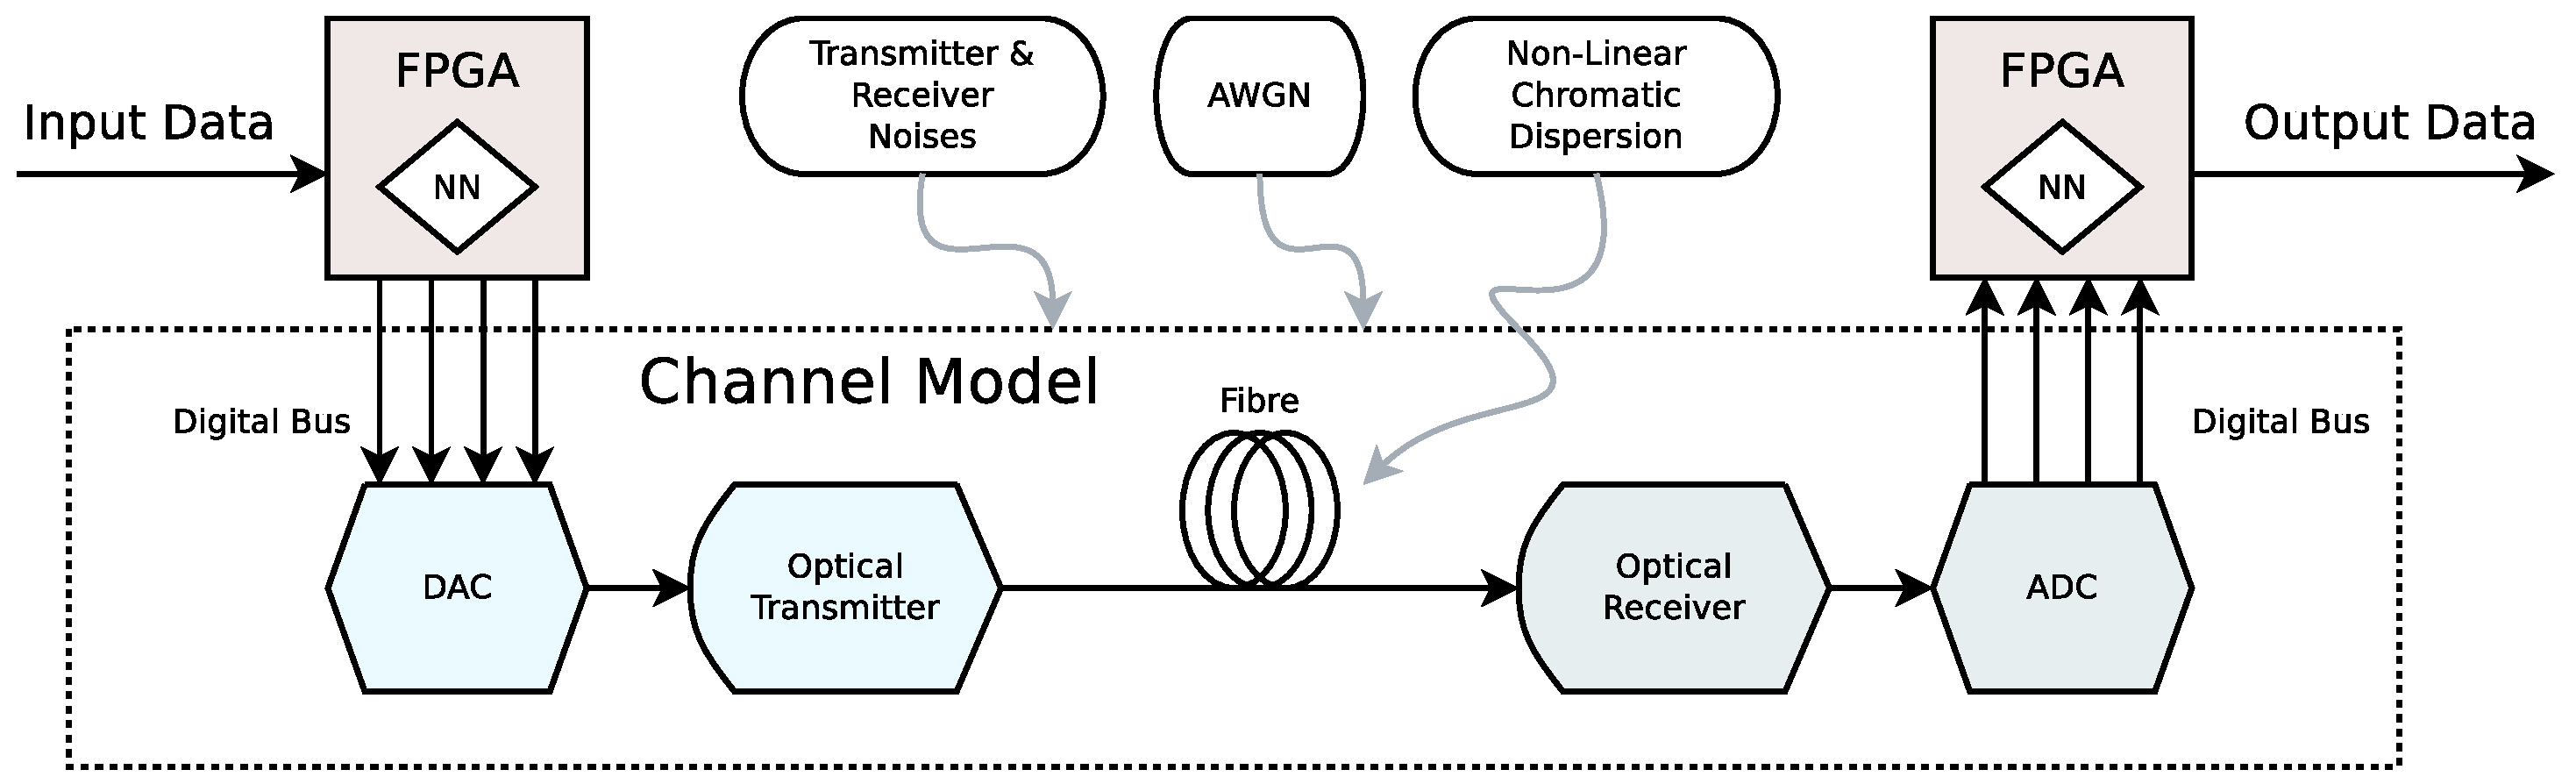
\includegraphics[width=\linewidth]{graphics/overall_diagram2.eps}
	\caption{Simplifier overall system diagram without inside FPGA Neural Network (NN) back-propogation learning.}
	\label{fig:overall}	
\end{figure}

\subsection{Choosing an Appropriate Neural Network Architecture}

The modulation scheme as well as the encoding of the bits will be learned for the specific communication channel by a neural network at the transmitter. Likewise, at the receiving end of the communication system, a separate neural network will decode the received signal into a stream of bits. A suitable neural network architecture must be chosen for each of the applications. 
\\
\\
The study carried out in \autocite{8664650} features a Convolutional Neural Network (CNN) at the transmitting and receiving end of the communication system. Similar to our own project, the paper describes an end to end neural network implementation for the communication system. The channel used in the simulations is an Additive White Gaussian Noise (AWGN) model and does not consider potential non-linearities introduced in the channel. On the contrary, \autocite{6975096} describes a Multi-Layer Perceptron (MLP) based Non-Linear Equalizer(NLE) at the receiver for an optical communication system. As this paper, clearly discusses the optical communication channel, it may be useful in deciding on a suitable neural network at the transmitter. It should be noted that the paper describes an equalizer and not a demodulator/decoder. 
\\
\\
Further research and literature review needs to be done into different architectures that are available and the requirements that need to be met by the transmitter and receiver of the communication channel. Depending on the chosen neural network architecture, a suitable FPGA will need to be decided on as well. Different architectures may demand different levels of hardware resources.

\subsection{Simulating the Communication Channel and Proposed Transmitter/Receiver}

The transmitting and receiving end as well as the channel itself need to be simulated as a channel model. The neural networks will most likely be implemented using the TensorFlow package with python. The different characteristics of the channel need to be included in the model to ensure that it sufficiently represents how a transmitted signal would be altered by a real optical fibre communication channel. \autocite{8433895} describes a potential model for the optical communication system. This model includes a low-pass filter (LPF) to account for the finite bandwidth of read hardware, a digital to analogue converter (DAC), an analogue to digital converter (ADC), a Mark-Zehnder modulator (MZM), photo-conversion by a photodiode, Gaussian noise as well as the optical fibre transmission itself. We will need to decide on the communication channel configuration that we wish to simulate as well as the data-rate of the communication system. 

This simulation could replace channel model which would look as a back box while training Neural Networks.

\subsection{Implementing the Neural Networks on a FPGA}

Implementing Neural Network on FPGA raises multiple problems that need to be solved.
 
\subsubsection{Floating-point vs fixed-point arithmetic}
FPGA internal data structure has number of trade-off that need to be decided on
\begin{itemize}
	\item \textbf{Floating-point} - allows high precision however are slower are require more resources. Native to other neural networks implemented in software.
	\item \textbf{Fixed-point} - introduce quantisation noise. Might be insufficient with very small or large values. Also requires deciding on sufficient bits size.
\end{itemize}
Preliminary research shows that fixed-point neural network implementation on FPGA achieves over 12x greater in speed, over 13x smaller in area, therefore allows far greater processing density \autocite{omondi_rajapakse_2006}. Therefore, further investigation needs to be done in order to determinate if fixed-point data structure is sufficient.

\subsubsection{Required FPGA resources}
 Depending on implemented Neural Network, its size, used data structure, a suitable FPGA board needs to selected. 
 
 Option to use multiple FPGA boards that would be linked with fast communication protocols will be also considered, including overall board architecture.

\subsubsection{Neural Network optimisations in FPGA} 
There are a number of research papers that include some optimisations to implement Neural Networks on FPGA: 
\begin{itemize}
	\item Feed forward ANN on FPGA \autocite{7011454}
	\item ANN based PID controller on FPGA \autocite{5328349}
\end{itemize}
Further research will be done to find optimal implementation of Neural Network in HDL.

\subsection{Training and Testing the System using an Optical Fibre Communication System}

If time and circumstance permits the project could conclude by testing the designed system using an experimental setup to simulate the communication channel as opposed to a computer model. This would bring light to discrepancies between the real-life setup and the simulated model. As well as that, it would validate that the design works as well in an experimental setup as it does in simulation. The neural network could be trained at different lengths of fibre and observed to see how the learned parameters as well as the bit error rate differ to traditional methods of encoding/decoding. 
